%Para este capítulo se usará la abreviatura "conex".
\chapter{Conexión}
\label{conex}

La noción de conexión es otra más de las nociones que ya conocíamos en $\R^n$ que pueden generalizarse a un espacio topológico arbitrario. Un conjunto es, intuitivamente, conexo, si está hecho ``de una sola pieza''. 

\section{Definición y propiedades}

Empezaremos viendo, por supuesto, la definición, y una serie de caracterizaciones equivalentes.

\begin{defi}[Conexión]
	$\X$ es \tbi[espacio!conexo|see{conexo}]{conexo} \indexg{conexo} si no es unión de dos abiertos disjuntos no vacíos, esto es, no existen $U,V\neq\emptyset$, abiertos, tales que $U\cap V=\emptyset$ y $X=U\cup V$.
\end{defi}

\begin{obs}[Conexión en subespacios]
	De nuevo, como con compacidad, la conexión en un subconjunto no necesita una definición alternativa. Dado $\mc{Y}\subset\X$, simplemente decimos que $\mc{Y}$ es conexo si lo es entendido como espacio equipado con la topología relativa. Nótese que esta definición es equivalente a la mucho más rebuscada que dábamos en $\R^n$, que involucraba abiertos relativos.
\end{obs}

\begin{prop}[Definiciones equivalentes de conexión]
	Sea un espacio topológico $\X$. Las siguientes afirmaciones son equivalentes:
	\begin{enumerate}
		\item $\X$ es conexo.
		\item $\X$ no es unión de dos cerrados disjuntos no vacíos, esto es, no existen $F,G\neq\emptyset$, cerrados, tales que $F\cap G=\emptyset$ y $X=F\cup G$.
		\item No hay ningún conjunto abierto y cerrado no trivial, esto es, $\nexists U$ abierto y cerrado tal que $U\neq\emptyset$ y $U\neq\X$.
	\end{enumerate}
\end{prop}

\begin{exa}
	En $\R$, los conexos son los intervalos. En efecto, si $A\subset\R$ no es un intervalo, entonces por definición $\exists a\notin A$ tal que $\inf A< a < \sup A$. Entonces, $(-\infty, a)\cap A)$ y $(a,\infty)\cap A$ son dos abiertos disjuntos no vacíos cuya unión contiene a $A$.
\end{exa}

Ahora, vamos a repasar brevemente las propiedades que ya conocíamos de conjuntos conexos.

\begin{prop}[Imagen continua]
	\label{conex_prop_im_continua}
	La imagen continua de un conexo es un conexo.
	
	\begin{proof}
		Sea $\X$ conexo, $f:\X\to\mc{Y}=f(\X)$ continua. Entonces queremos ver que $\mc{Y}$ es conexo. Para ello vamos a ver el contrarrecíproco: si $\mc{Y}$ no es conexo $\X$ tampoco.
		
		Si existiera $A\subset\mc{Y}$ abierto y cerrado no trivial (esto es, que no es ni el vacío ni el total), entonces por ser $f$ continua $f^{-1}(A)$ es también abierta y cerrada, y por ser $f$ sobreyectiva $f^{-1}(A)$ no es el vacío ni el total. Por tanto $\X$ no es conexo.
	\end{proof}
\end{prop}

% NOTA: no he nombrado el teorema como teorema del pivote porque buscado en internet sólo salía en la página de Ruiz con ese nombre. En demás libros que he visto no tiene nombre.
\begin{theo}
	\label{conex_theo_pivote}
	Sea $\{A_i\}_{i\in I}$ una familia de conexos de $\X$ y existe $a\in\bigcap_{i\in I} A_i$. Entonces $\bigcup_{i\in I} A_i$ es conexo.
	
	\begin{proof}
		Supongamos que existe $S\subset\bigcup_{i\in I} A_i$ abierto y cerrado. Vamos a ver que necesariamente es el vacío o el total. Entonces, para cada $i\in I$ tenemos que $S\cap A_i\subset A_i$ es abierto y cerrado en $A_i$. Ahora, como $A_i$ es conexo, $S\cap A_i$ tiene que ser necesariamente el vacío o el total, para cada $i\in I$. Distinguimos pues dos casos:
		\begin{enumerate}
			\item Si $S\cap A_i=\emptyset\;\forall i\in I$, entonces $S=\emptyset$ y ya está.
			\item Si $\exists i\in I$ tal que $S\cap A_i=A_i$, entonces $\exists a\in S\cap A_i$ que por hipótesis verifica que $a\in S\cap A_j$ para todo $j\in I$. Entonces ninguno de los $S\cap A_j$ es vacío, y por tanto $S\cap A_j=A_j\;\forall j\in I$, es decir, $S=\bigcup_{i\in I} A_i$. \qedhere
		\end{enumerate}
	\end{proof}
\end{theo}

Este teorema es extremadamente útil para garantizar la conexión de un sinnúmero de conjuntos, y genera un gran abanico de corolarios y consecuencias. Aquí vamos a detallar algunos que se usan con frecuencia.

\begin{cor}
	\label{conex_cor_pivote_corte_comun}
	Sea $\{A_i\}_{i\in I}$ una familia de conexos que cumple que $\exists i_0\in I$ tal que $A_{i_0}\cap A_i\neq\emptyset\;\;\forall i\in I$. Entonces $\bigcup_{i\in I} A_i$ es conexo. En particular, el resultado se verifica si la familia cumple que $A_i\cap A_j\neq\emptyset\;\;\forall i\neq j$.
	
	\begin{proof}
		Como $A_i\cap A_{i_0}\neq\emptyset$ por hipótesis, podemos aplicar el teorema \ref{conex_theo_pivote} para cada $i\in I$, y por tanto cada $A_{i_0}\cup A_i$ es conexo. Ahora, escribimos:
		\[\bigcup_{i\in I} A_i = \bigcup_{i\in I} (A_i\cup A_{i_0})\]
		y como todos comparten los elementos de $A_{i_0}$, podemos aplicar el teorema de nuevo.
	\end{proof}
\end{cor}

\begin{cor}
	Sea una cadena $\{A_i\}_{i=1}^n$ de conexos que verifica que $A_i\cap A_{i+1}\neq\emptyset$. Entonces $\bigcup_{i=1}^n A_i$ es conexo.
	
	\begin{proof}
		Por inducción, se aplica el teorema \ref{conex_theo_pivote} a $A_1\cup A_2$, $(A_1\cup A_2)\cup A_3$, ..., $\left(\bigcup_{i=1}^k A_i\right)\cup A_{k+1}$.
	\end{proof}
\end{cor}

\begin{obs}
	El corolario anterior también se verifica si la sucesión de conjuntos es numerable, pero no lo vamos a probar aquí.
	% AQUÍ VIENE PROBADO http://dbfin.com/topology/munkres/chapter-3/section-23-connected-spaces/problem-2-solution/
\end{obs}

El siguiente resultado, aunque también es consecuencia del teorema \ref{conex_theo_pivote}, es más que un mero corolario y merece la categoría de teorema por sí mismo.

\begin{theo}
	Sea $A$ conexo, $B$ tal que $A\subset B\subset\adher{A}$. Entonces $B$ es conexo. En particular $\adher{A}$ es conexo.
	
	\begin{proof}
		Como podemos escribir:
		\[B=\bigcup_{b\in B\setminus A} (A\cup\{b\}) \]
		y todos comparten un punto, entonces basta probar que cada $A\cup\{b\}\subset\adher{A}$ es conexo, pues en ese caso el teorema \ref{conex_theo_pivote} nos garantiza la conexión de $B$.
		
		Supongamos que $\exists C\subset A\cup\{b\}$ abierto y cerrado y no trivial. Entonces, $C\cap A\subset A$ y es abierto y cerrado en $A$. Como $A$ es conexo distinguimos dos casos:
		
		\begin{itemize}
			\item Si $C\cap A=\emptyset$, entonces $C=\{b\}$ y por tanto $\{b\}$ es abierto, luego, como el entorno $\{b\}$ de sí mismo no corta con $A$, $b\notin\adher{A}$, lo cual es una contradicción.
			\item Si $C\cap A=A$, $C=A$ y por tanto $A$ es cerrado, pero $b\notin A=\adher{A}$, que de nuevo es una contradicción. \qedhere
		\end{itemize}
	\end{proof}
\end{theo}

Aprovechando los resultados anteriores podemos garantizar la conexión de un buen número de espacios.

\begin{exa} Veamos algunos ejemplos de conjuntos conexos:
	\begin{enumerate}
		\item En $\R^n$, se dice que un conjunto es \tbi{convexo} si para cada par de puntos el segmento que los une también está en el conjunto; y se dice que es \tbi{estrellado} si existe un punto tal que el segmento de él a cualquier otro está en el conjunto. Si un conjunto es convexo entonces es estrellado, y si es estrellado entonces es conexo. Además, las implicaciones recíprocas no se verifican.
		
		En efecto, un conjunto $A$ estrellado se puede escribir como:
		\[A=\bigcup_{a\in A} [a_0, a]\]
		para cierto $a_0\in A$. Cada segmento $[a_0,a]$ es conexo por la proposición \ref{conex_prop_im_continua}, al ser la imagen del intervalo conexo $[0,1]$ por la aplicación:
		\[t\mapsto (1-t)a_0+ta\]
		y por tanto, por el teorema \ref{conex_theo_pivote}, como todos comparten el punto $a_0$ su unión es conexa.
		
		Nótese que ni la convexidad ni ser estrellado son propiedades topológicas; ambas son propiedades métricas: su definición solo tiene sentido en un espacio que, al menos, tenga definida una distancia.
		
		\item Una circunferencia en $\R^2$ es conexa, pero no es estrellada. En efecto, es conexa por ser la imagen de $[0,2\pi]$ por la aplicación $t\mapsto (\cos t, \sen t)$.
		
		\item El grafo de la función $\sin\frac{1}{x}$ para $x>0$, que escribimos:
		\[C = \left\{\left(x,\sin\frac{1}{x}\right)\midc x>0\right\}\]
		es conexo por ser la imagen continua de $(0,\infty)$ por la aplicación:
		\[x\mapsto \left(x,\sin\frac{1}{x}\right)\]
		
		Lo que es más interesante, para cualquier $a\in [-1,1]$ se verifica que $\{(0,a)\}$ es adherente a $C$ y por tanto que $C\cup\{(0,a)\}$ es conexo.
		
		\item Consideramos el conjunto:
		\[C = \big(\{0\}\times (0,1]\big) \cup \left(\bigcup_{n\in\N} [0,1]\times\left\{\frac{1}{n}\right\}\right) \]
		que es unión de segmentos horizontales cada vez más juntos y de un segmento vertical. Este es trivialmente conexo por el corolario \ref{conex_cor_pivote_corte_comun}. Lo particular es que si unimos a $C$ el segmento horizontal:
		\[(0,1)\times\{0\}\]
		sigue siendo conexo por ser adherencia de $C$. \qedhere
	\end{enumerate}
\end{exa}

Completamos esta sección con una propiedad interesante garantizada por la conexión.

\begin{lem}
	Sea $\X$ conexo y $\{U_i\}_{i\in I}$ una familia de abiertos, de forma que $\X=\bigcup_{i\in I} U_i$. Dos puntos cualesquiera $x,y\in\X$ se pueden conectar mediante una cadena finita $\{U_{i_k}\}_{k=1}^n$ de abiertos de la familia que verifique que $U_{i_k}\cap U_{i_{k+1}}\neq\emptyset$.
	
	\begin{proof}
		Sea $A=\{z\in\X \midc \text{existe una cadena de } x \text{ a } z \}$. $A$ es claramente no vacío, puesto que $x\in A$. Entonces, una forma de ver que $\X=A$, que es lo que queremos encontrar, es comprobar que $A$ es abierto y cerrado, puesto que entonces solo puede ser el total (pues hemos visto que es no vacío).
		
		\begin{itemize}
			\item Veamos que $A$ es abierto. En efecto, dado $z\in A$, queremos ver que existe un abierto $U$ tal que $z\in U\subset A$. Pero basta con tomar el último de la cadena, que ya cumple estas condiciones.
			
			\item Ahora veamos que es cerrado. En efecto, si $z\in\adher{A}$, existe un abierto $U_{i_0}$ tal que$U_{i_0}\cap A\neq\emptyset$. Entonces, tomamos un punto $y$ de la intersección, y como está en $A$ hay una cadena de $x$ a $y$. Uniendo $U_{i_0}$ a la cadena tenemos una cadena de $x$ a $z$, y por tanto $z\in A$, luego $A=\adher{A}$. \qedhere
		\end{itemize}
	\end{proof}
\end{lem}

\begin{obs}
	En particular, puedo recubrir cualquier abierto conexo de $\R^n$ por bolas, y por tanto existe una cadena de bolas que une cualquier par de puntos. Si tomo un punto en cada intersección entre bolas consecutivas de la cadena y los uno, tengo una poligonal que conecta los dos puntos. Entonces, si $C\subset\R^n$ es abierto, $C$ es conexo si y solo si es conexo por poligonales (la definición de conexión por poligonales y la implicación inversa corresponden a cálculo diferencial).
\end{obs}

%Tablas comportamiento topológico. Añado aquí también las de conexión por caminos, dado que no está aun el tema.

\section{Comportamiento topológico}

\begin{table}[h]
	\centering
	\begin{tabular}{l|l|l|l|l|}
		\cline{2-5}
		& \textbf{Subespacios}    & \textbf{Cociente}       & \textbf{Producto}       & \textbf{Suma}           \\ \hline
		\multicolumn{1}{|c|}{\textbf{Conexión}} & \multicolumn{1}{c|}{No} & \multicolumn{1}{c|}{Sí*} & \multicolumn{1}{c|}{Sí} & \multicolumn{1}{c|}{No} \\ \hline
	\end{tabular}
	\caption{Tabla resumen de conexión.}
	\label{Tabla_conexion}
\end{table}

\begin{table}[h]
	\centering
	\begin{tabular}{l|l|l|l|l|}
		\cline{2-5}
		& \textbf{Subespacios}                                                                      & \textbf{Cociente}       & \textbf{Producto}       & \textbf{Suma}           \\ \hline
		\multicolumn{1}{|c|}{\textbf{\begin{tabular}[c]{@{}c@{}}Local\\ conexión\end{tabular}}} & \multicolumn{1}{c|}{\begin{tabular}[c]{@{}c@{}}Sí, en el caso\\ de abiertos\end{tabular}} & \multicolumn{1}{c|}{Sí} & \multicolumn{1}{c|}{Sí} & \multicolumn{1}{c|}{Sí} \\ \hline
	\end{tabular}
	\caption{Tabla resumen de local conexión}
	\label{Tabla_localconexion}
\end{table}

\begin{table}[h]
	\centering
	\begin{tabular}{c|c|c|c|c|}
		\cline{2-5}
		\multicolumn{1}{l|}{}                                                                                  & \multicolumn{1}{l|}{\textbf{Subespacios}}                             & \multicolumn{1}{l|}{\textbf{Cociente}} & \multicolumn{1}{l|}{\textbf{Producto}} & \multicolumn{1}{l|}{\textbf{Suma}} \\ \hline
		\multicolumn{1}{|c|}{\textbf{\begin{tabular}[c]{@{}c@{}}Conexo por\\ caminos\end{tabular}}}            & No                                                                    & Sí                                     & Sí                                     & No                                 \\ \hline
		\multicolumn{1}{|c|}{\textbf{\begin{tabular}[c]{@{}c@{}}Localmente conexo\\ por caminos\end{tabular}}} & \begin{tabular}[c]{@{}c@{}}Sí, en el caso \\ de abiertos\end{tabular} & Sí                                     & Sí                                     & Sí                                 \\ \hline
	\end{tabular}
	\caption{Tabla resumen de conexión por caminos}
	\label{Tabla_conexion_caminos}
\end{table}

\begin{figure}[h!]
	\centering
	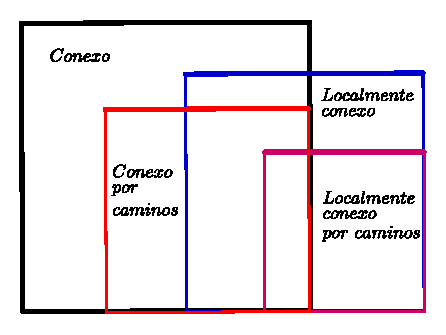
\includegraphics[scale = 1]{img/Comparacion_conexion}
\end{figure}
